\chapter{Edge disjoint path problem}

Some readers may already know what is edge disjoint path problem and also some basic algorithms. But we will have a brief introduction to this topic.

\begin{itemize}
	\item \textbf{INPUT}: $G=(V,E)$ and $(s_{i}, t_{i}) \in V^2$ for all $i \in [k]$.
	\item \textbf{OUTPUT}: $I \subseteq [k]$ and an $s_{i}-t_{i}$ path $P_{i}$ for each $i \in I$, s.t. the selected paths are edge disjoint.
	\item \textbf{OBJECTIVE}: $\max |I|$.
\end{itemize}

It is known that this particular problem is NP-hard. So we will again show some approximation to this problem. \textit{Note: for any fix $k$ it is solvable in polynomial time on undirected graph. But for directed graphs it is NP-hard for $k = 2$.} We will introduce an greedy algorithm that has an parameter.

\begin{algorithm}
	\caption{Greedy algorithm with a catch for parameter $\sqrt{m}$}
	\begin{algorithmic}[1]
		\State $I = \emptyset$
		\While{$\exists i \notin I$ and $\exists s_{i}-t_{i}$ path in $G$, s.t. $|P_{i}| \leq \sqrt{m}$}
			\State $I = I \cup \{i\}$, keep $P_{i}$, $G = G \setminus P_{i}$
		\EndWhile
	\end{algorithmic}
\end{algorithm}

We will denote $OPT$ as the optimal solution of the problem. It will be either a set of paths or set of indexes. Then we will denote $OPT_{S} = \{P \in OPT \mid |P| \leq \sqrt{m}\}$, where the length of a path is set as the number of edges. Then $OPT_{L} = OPT \setminus OPT_{S}$ and $ALG$ as the set given by the algorithm.

Now take the set $OPT_{S} \setminus ALG$. That is path between $s_{i}$ and $t_{i}$ is in this set if there exists $s_{j}-t_{j}$ path obtained by the algorithm which shares an edge. This path has length at most $\sqrt{m}$ and there are $|ALG|$ paths. Thus altogether $|OPT_{S} \setminus ALG| \leq \sqrt{m} |ALG|$.

Next we may see that $|OPT_{L}| \leq \sqrt{m}$, because we have $m$ edges and each one of them is at least $\sqrt{m}$ long. Now we may conclude altogether following result.

$$
|OPT| \leq |OPT_{L}| + |OPT_{S} \setminus ALG| + |ALG| \leq O(\sqrt{m}) |ALG|
$$

Now one can see where the catch in the algorithm is. Consider that there are no such short paths. The algorithm will output no path at all. To fix this we need to change the algorithm such that it will always output at least one path. If there is none then $OPT$ is 0 as well.

\begin{algorithm}
	\caption{Greedy ($\sqrt{m}$)}
	\begin{algorithmic}[1]
		\State $I = \emptyset$
		\While{$\exists i \notin I$ and $\exists s_{i}-t_{i}$ path in $G$, s.t. $|P_{i}| \leq \sqrt{m}$}
		\State $I = I \cup \{i\}$, keep $P_{i}$, $G = G \setminus P_{i}$
		\EndWhile
		\If{\textcolor{purple}{$I = \emptyset$}}
			\State \textcolor{purple}{Connect any $s_{i}-t_{i}$ path if possible.}
		\EndIf
	\end{algorithmic}
\end{algorithm}

Thus we have shown an algorithm that is a $\sqrt{m}$-approximation. Now we consider running the same algorithm but we change the parameter from $\sqrt{m}$ to $n^{2/3}$. Can we obtain $n^{2/3}$-approximation?

\begin{thm}[Khana, Chedari]
	Given an instance of the sum multi-commodity flow problem $G =(V,E), (s_{i}, t_{i}) \in V^2$ for all $i \in [k]$ such that $(\forall i) d(s_{i}, t_{i}) \leq l$, then the max multi-commodity flow is $O(\frac{n^2}{l^2})$.
\end{thm}

Before proving this we will show the consequences for our problem. Lets use the algorithm Greedy$(n^{2/3})$. Assume there $\exists P_{i} \in ALG, |P_{i}| \leq n^{2/3}$. Otherwise we use the theorem on the network obtained by $G$ and setting all capacities to one. Then all edges are at least $n^{2/3}$ length so we get the max multi-commodity flow is $O(\frac{n^{2}}{n^{4/3}}) = O(n^{2/3})$. Therefore it means if we choose just one path the approximation ratio will still be $O(n^{2/3})$.

Denote $OPT_{easy} = \{P \in OPT \mid \exists Q \in ALG : Q \cap P \neq \emptyset\}$. With this we know that $|OPT_{easy}| \leq n^{2/3} |ALG|$ by the same argument as it was already mentioned before.

We will look at $\forall (s_{i}, t_{i}) \in (OPT \setminus OPT_{easy}) \setminus ALG$. What can we say about such $d(s_{i}, t_{i})$ at the end of the loop of the algorithm. Clearly because it was not chosen either there is some intersection with another path, but this is remove by $OPT_{easy}$, so the other option is only that $d(s_{i}, t_{i}) > n^{2/3}$. Hence $|(OPT \setminus OPT_{easy}) \setminus ALG| \leq O(n^{2/3})$ by the theorem and the same argument which was already mentioned. Altogether we have:

$$
|OPT| \leq |OPT_{easy}| + |(OPT \setminus OPT_{easy}) \setminus ALG| + |ALG| = O(n^{2/3}) |ALG|
$$

Now we only need to proof the theorem since it is the base of our arguments for obtaining $O(n^{2/3})$-approximation algorithm.

\begin{proof}
	We will split the vertices into two sets:
	
	\begin{enumerate}
		\item \textbf{low degree vertex} are when $\deg(v) \leq \frac{6 n}{l}$
		\item \textbf{high degree vertex} are when $\deg(v) > \frac{6 n}{l}$
	\end{enumerate}
	
	Also we will assume $l$ is a multiple of 6. Otherwise it get lost in the $O$ notation. To finish the proof we will use an observation.
	
	\begin{observ}
		Any $s_{i}-t_{i}$ path (denote it as $s-t$) uses at least $l/6$ low degree vertices.
	\end{observ}
	
	\begin{proof}[Proof of observation]
		Consider running BFS on the graph starting from $s$. We denote $L_{i} = \{u \in V : d(s,u) = i\}$. Note that edges are only within one layer or only between adjacent layers. Let $B_{i}$ be a block of three consecutive layers $\{L_{3i}, L_{3i+1}, L_{3i+2}\}$. Because the length to $t$ is at least $l$ then there is at least $l/3$ blocks. Assume that $< l/6$ layers consists of only low degree vertices. Otherwise the observation obviously holds. Now discard all blocks containing a layer of only low degree vertices. As there are $\geq l/3$ blocks at least $\geq l/6$ blocks remain. Then the smallest remaining block is of size $\leq \frac{n}{l/6} = 6n/l$ which can be seen by pigeonhole principle. For the vertices in the middle layer we know all neighbors are within the block. Therefore it is a low degree vertex. This is a contradiction because we still have a block having one layer with low degree vertices only.
	\end{proof}
	
	Now for the theorem we know a \textbf{unit} of flow between any pair $s_{i}-t_{i}$ consumes $\mathbf{\Omega(l)}$ cpacity of edges adjacent to low degree vertices. And the total capacity adjacent to low degree vertices is $\leq n \deg(v) \leq n (6n/l) = O(n^2/l)$. Which gives us $O(n^2/l^2)$.
\end{proof}

This is an example of greedy algorithm and the fact that using it with different parameter may result in better approximation, but the analysis is way harder. We also saw using flows to limit paths, but this has also its limits. We will show a counterexample a graph called \textbf{Brick wall}.

\begin{figure}[!ht]\centering
	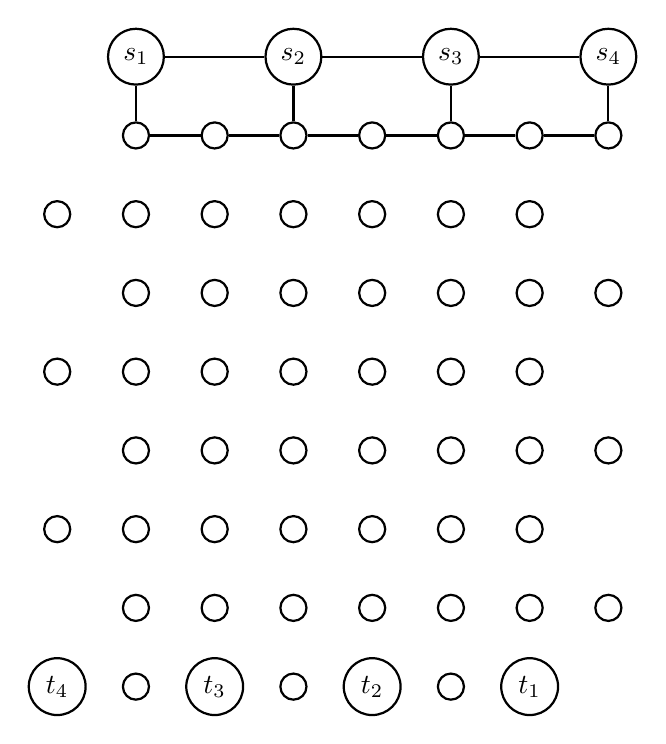
\begin{tikzpicture}[node distance={10mm}, thick, main/.style = {draw, circle}]
		\node[main] (1) {$s_{1}$};
		\node[main] (5) [below of=1] {};
		\node[main] (6) [right of=5] {};
		\node[main] (7) [right of=6] {};
		\node[main] (2) [above of=7] {$s_{2}$};
		
		\node[main] (8) [right of=7] {};
		\node[main] (9) [right of=8] {};
		\node[main] (3) [above of=9] {$s_{3}$};
		
		\node[main] (10) [right of=9] {};
		\node[main] (11) [right of=10] {};
		\node[main] (4) [above of=11] {$s_{4}$};
		
		\node[main] (13) [below of=5] {};
		\node[main] (12) [left of=13] {};
		\node[main] (14) [right of=13] {};
		\node[main] (15) [right of=14] {};
		\node[main] (16) [right of=15] {};
		\node[main] (17) [right of=16] {};
		\node[main] (18) [right of=17] {};
		
		\node[main] (22) [below of=13] {};
		\node[main] (23) [right of=22] {};
		\node[main] (24) [right of=23] {};
		\node[main] (25) [right of=24] {};
		\node[main] (26) [right of=25] {};
		\node[main] (27) [right of=26] {};
		\node[main] (28) [right of=27] {};
		
		\node[main] (33) [below of=22] {};
		\node[main] (32) [left of=33] {};
		\node[main] (34) [right of=33] {};
		\node[main] (35) [right of=34] {};
		\node[main] (36) [right of=35] {};
		\node[main] (37) [right of=36] {};
		\node[main] (38) [right of=37] {};
		
		\node[main] (42) [below of=33] {};
		\node[main] (43) [right of=42] {};
		\node[main] (44) [right of=43] {};
		\node[main] (45) [right of=44] {};
		\node[main] (46) [right of=45] {};
		\node[main] (47) [right of=46] {};
		\node[main] (48) [right of=47] {};
		
		\node[main] (53) [below of=42] {};
		\node[main] (52) [left of=53] {};
		\node[main] (54) [right of=53] {};
		\node[main] (55) [right of=54] {};
		\node[main] (56) [right of=55] {};
		\node[main] (57) [right of=56] {};
		\node[main] (58) [right of=57] {};
		
		\node[main] (62) [below of=53] {};
		\node[main] (63) [right of=62] {};
		\node[main] (64) [right of=63] {};
		\node[main] (65) [right of=64] {};
		\node[main] (66) [right of=65] {};
		\node[main] (67) [right of=66] {};
		\node[main] (68) [right of=67] {};
		
		\node[main] (73) [below of=62] {};
		\node[main] (72) [left of=73] {$t_{4}$};
		\node[main] (74) [right of=73] {$t_{3}$};
		\node[main] (75) [right of=74] {};
		\node[main] (76) [right of=75] {$t_{2}$};
		\node[main] (77) [right of=76] {};
		\node[main] (78) [right of=77] {$t_{1}$};
		%12 13 14 15 16 17 18
		%22 23 24 25 26 27 28
		
		\draw (1) -- (2);
		\draw (2) -- (3);
		\draw (3) -- (4);
		
		\draw (1) -- (5);
		\draw (2) -- (7);
		\draw (3) -- (9);
		\draw (4) -- (11);
		
		\draw (5) -- (6);
		\draw (6) -- (7);
		\draw (7) -- (8);
		\draw (8) -- (9);
		\draw (9) -- (10);
		\draw (10) -- (11);
	\end{tikzpicture}
	\caption{Example of a \textbf{brick wall} graph for $k = 4$.}
	\label{brick-wall}
\end{figure}

The graph you may see at the picture \ref{brick-wall} is planar. Also it can be generalized to $k$ where there are $k$ pairs of bricks underneath. The edge disjoint problem optimum is 1, which we can see on picture \ref{edg}. And the max multi flow optimum is at least $k/2 = O(\sqrt{n})$, which can be seen on picture \ref{max-flow}.


\begin{figure}[!ht]\centering
	\caption{Edge disjoint problem.}
	\label{edg}
\end{figure}

\begin{figure}[!ht]\centering
	\caption{Max multi flow optimum.}
	\label{max-flow}
\end{figure}